%% The following is a directive for TeXShop to indicate the main file
%%!TEX root = diss.tex

\chapter{Discussion and conclusions}
\label{chap:conclusion}

This dissertation set out to examine the influence of listener attentional sets on perceptual learning.
Perceptual learning is a phenomenon common to many fields involved in cognitive science.
How perceptual learning generalizes to new contexts, however, is quite different across paradigms.
Perceptual learning in psychophysics is the process of a perceiver aligning their senses to the world.
Perceptual learning in speech perception is the process by which perceivers align their perceptual system to an interlocutor to facilitate understanding.

I argue that perceptual learning as a mechanism is shared between linguistic and non-linguistic domains.
However, psychophysics paradigms employ primarily perception-oriented attentional sets, while speech perception paradigms employ both perception-oriented and comprehension-oriented attentional sets.
Perception-oriented attentional sets in all domains leads to less generalized learning.
Conversely, comprehension-oriented attentional sets lead to more generalized learning.
The first two experiments of this dissertation implement a standard lexically-guided perceptual learning paradigm -- a lexical decision task -- but with manipulations promoting perception-oriented attentional sets.
Even in a comprehension-oriented lexical decision task, promoting more perception-oriented attentional sets leads to less generalized learning.
These results provide a crucial link between fully comprehension-oriented perceptual learning in the lexically-guided paradigm and fully perception-oriented perceptual learning in visually-guided paradigms.
The remainder of this chapter first summarizes the results of the dissertation as they relate to specificity and generalization in the perceptual learning literature.
The four manipulations used to promote the different attentional sets are then examined, followed finally by implications for models of cognition and psycholinguistics.

\section{Specificity and generalization in perceptual learning}

The results of this dissertation speak to the dichotomy between specificity and generalization found in the perceptual learning literature. 
In Experiment 1, participants had larger perceptual learning effects when they were exposed to ambiguous sounds later in the words rather than at the beginning of words (e.g. \emph{carousel} versus \emph{cement}). 
And yet, the testing continua consisted of stimuli with the sibilant at the beginnings of words, which are more similar to the exposure tokens beginning with the ambiguous sound.
Exposure that matched the word position of the categorization (word-initial) showed no greater perceptual learning effects than word-medial exposure.
Perceptual learning, therefore, occurred at a level of abstraction that is usually not assumed in perceptual learning studies.
Most lexically-guided perceptual learning studies attempt to make the exposure tokens and the categorization similar -- and in some cases, the same -- in order to maximize exposure-specificity effects.
The results of this dissertation show that listeners show perceptual learning effects from stimuli with large degrees of coarticulation (i.e., in the middle of the word) to stimuli without as much coarticulation. 
In some cases, perceptual learning is greatest in precisely the cases where coarticulatory effects differed from exposure to test.
One aspect that was not tested in the current studies is exposure-specificity at the level of the item.
Perhaps a more perception-oriented attentional set would show greater perceptual learning on the specific exposure items.

The effect of attentional set manipulations in Experiments 1 and 2 suggest that when listeners adopt more perceptually-oriented attentional sets, even within tasks that are oriented toward comprehension, generalization of perceptual learning to new forms is inhibited.
Lexically-guided perceptual learning is more likely to be expanded to new contexts  than visually-guided perceptual learning \citetext{\citealp{Norris2003, Kraljic2008a,Reinisch2014}, but see \citealp{Mitterer2013}}.
Visually-guided and psychophysical perceptual learning paradigms often have highly repetitive stimuli with little variation.  
Both of these aspects add to the monotony of the task and the likelihood of perception-oriented attentional sets \citep{Cutler1987}.

Lexically-guided perceptual learning, on the other hand, requires very few instances to affect the perceptual system.
The standard number is around 20 ambiguous tokens within 200 trials, but as few as 10 ambiguous tokens have been shown to have comparable effects \citep{Kraljic2008}.
A consequence of the proposed attention mechanism is that it nicely captures the differences in numbers of stimuli across comprehension-oriented and perception-oriented tasks.
Tokens heard under comprehension-oriented attentional sets should have a relatively large effect on the perceptual system as compared to tokens heard under a perception-oriented attentional set.
A single token updating a more abstract representation will generalize more than many repetitions updating fine-grained episodic representations.
From this, we could predict that word endorsement rate and category boundary shift would be less linearly correlated the more comprehension-oriented participants are.
This prediction is borne out by the lack of correlation between word endorsement rate and cross-over point in Experiment 1 in the Word-final/No Attention condition.
This condition is predicted to have the most comprehension-oriented attentional set of the conditions, and here is the only instance in Experiment 1 where a significant correlation between word endorsement rate and cross-over point is not present.
Participants in this condition have relatively high cross-over points that do not depend as much on the sheer number of tokens endorsed.

\section{Effect of increased linguistic expectations}

The conditions of Experiment 1 that are most similar to previous lexically-guided perceptual learning paradigms are those with no explicit instructions about the /s/ category.
In these conditions, increasing linguistic expectations through lexical bias resulted in larger perceptual learning effects.
I argue that the increased perceptual learning is due to increased maintenance of comprehension-oriented attentional sets by participants in the Word-medial condition.
The participants exposed to a modified /s/ category at the beginnings of words would be more likely to have their attention drawn to the atypicality of the modified /s/ category.
There are two potential scenarios for how this would have affected participants.
In the first, ``normal'' word processing would proceed with the perception of the modified /s/ as part of comprehending the word, but the attentional set would not change.
In the second, processing the word would trigger an attentional set change that would get reinforced for each new modified /s/ encountered.
The experiments in this dissertation do not definitively answer which scenario is more likely, and it could be that different participants fall into different scenarios.
However, when participants were told about the ambiguity of the /s/, they do not behave any differently if the /s/ is word-initial or word-medial.
This similarity of behavioral patterning suggests the second scenario is more likely, and more perception-oriented attentional sets were adopted as a result of exposure to words beginning with a modified /s/ category.

Increasing linguistic expectations through semantic predictability did not increase perceptual learning.
In fact, there was a trend towards unpredictive sentences increasing perceptual learning.
Semantic predictability has previously been shown to affect perception-oriented tasks in a similar way as lexical bias \citep{Connine1987, Borsky1998}.
In Experiment 3, however, participants exposed to the modified /s/ category in high predictability sentences showed no perceptual learning effects at all.
While the Isolation condition (Word-medial condition in Experiment 1) was not significantly different from the Unpredictive condition of Experiment 3, there was a trend toward reduced perceptual learning when the modified sound category was embedded in a sentential context in general.
The lack of a perceptual learning effect from high predictability exposure sentences is reminiscent of studies that find no perceptual learning when a modified /s/ category is embedded in a /st\textturnr/ cluster that conditions that variation \citep{Kraljic2008a}.
In both cases, the modified category is embedded in a context that conditions increased variability.
However, there is a difference between the consonant cluster context and the semantic predictability context.
In the consonant cluster, there is a straightforward coarticulatory reason for /s/ to surface as more /\textesh/-like in /st\textturnr/ clusters, with the /s/ produced more in a postalveolar position due to the upcoming /\textturnr/.
For semantic predictability, there is no particular reason why a /s/ should surface more /\textesh/ like in high predictability sentences.
If high semantic predictability can be the attributed cause of /s/ surfacing as more /\textesh/-like, it seems reasonable that the range of acceptable productions for all categories would be expanded (as schematized in Figure~\ref{fig:distPred} of Chapter~\ref{chap:sent}).

Perceptual learning of nonnative accents is possible through hearing sentences of varying predictability \citep[and others]{Bradlow2008}.
However, the phonetic variability involved in those tasks reaches far beyond that involved here.  
The speaker producing the sentences in this dissertation is a native English speaker of the local dialect.
Even with the synthesis applied to the sound files, he is more intelligible than the speakers in studies involving nonnative accents.
The ease of comprehension of the speaker in this study might actually inhibit perceptual learning in sentences, because listeners can leverage so much of their perceptual experience with other speakers of the local dialect.

On the flip side, how nonnative listeners perceptually adapt to speech that varies in predictability is an interesting question as well.
Nonnative listeners do not benefit from high semantic predictability as much as native listeners \citep{Mayo1997}.
This tends to result in less accuracy for transcribing speech in noise.
As the sentences presented here did not include noise, the lessened benefit from semantic predictability might manifest differently.
If high predictability sentences are not as predictable for those listeners, they may show perceptual learning effects more similar to unpredictable sentences.


\section{Attentional control of perceptual learning}

The findings of Experiment 1 support the hypothesis that comprehension-oriented attentional sets produce larger perceptual learning effects than perception-oriented attentional sets.  
Although all participants showed perceptual learning effects, those exposed to the ambiguous sound with increased lexical bias only showed larger perceptual learning effects when the instructions about the speaker's ambiguous sound were withheld.  
Attention on the ambiguous sound equalized the perceptual learning effects across lexical bias.
However, in Experiment 2, there is no such effect of attention.
This suggests that ambiguous sounds farther away from the canonical production induce a more perception-oriented attentional set regardless of explicit instructions.

One question raised by the current results is whether perception-oriented attentional sets always result in decreased perceptual learning.  
The instructions used to focus the listener's attentional set framed the ambiguity in a negative way, with listeners being cautioned to listen carefully to ensure they made the correct decision.  
If the attention were directed to the ambiguous sound by framing the ambiguity in a positive way, would we still see the same pattern of results?
The current mechanism would predict that attention of any kind to signal properties would block the propagation of errors, reducing perceptual learning.
This prediction will be tested in future work.

Attention's role in perceptual learning may extend to the realm of sociolinguistics.  
In sociolinguistics, there are three categories of linguistic variables: indicators, markers, and stereotypes \citep{Labov1972}.
Of these, stereotypes are the most known to speakers of the dialect and speakers of other dialects.
If attention to perception inhibits perceptual learning, then perceptual learning to these stereotype linguistic variables would be inhibited relative to other variables.
Given the scale from indicators to markers to stereotypes is ordered in terms of speaker (or listener) awareness, the role of attention proposed in this dissertation would predict progressively less perceptual learning as awareness increases.
Salient social variants (i.e. r-lessness) have also been found to not be encoded as robustly as canonical productions \citep{Sumner2009}.
Would less salient social variants be learned easier?

\section{Category atypicality}

In Experiment 2, there was no effect of explicit instructions or lexical bias on perceptual learning, with a stable perceptual learning effect present for all listeners.
There are two potential, non-exclusive explanations for the lack of effects.
As stated above, the increased distance to the canonical production drew the listener's attention to the ambiguous productions, resulting in a perception-oriented attentional set.
The second potential explanation is that the productions farther from canonical produce a weaker effect on the updating of a listener's categories, as predicted from the neo-generative model in \citet{Pierrehumbert2002}.
This explanation is supported in part by the weaker correlation between word endorsement rate and cross-over point found in Experiment 2, and the findings of \citet{Sumner2011} where the highest rates of perceptual learning were found when the categories began more typical and gradually became less typical over the course of exposure.
This explanation could be tested straightforwardly by implementing the same gradual shift paradigm used in \citet{Sumner2011} with the manipulations used in this dissertation.

An interesting extension to the current findings would be to observe the perceptual learning effects in a cognitive load paradigm.  
Speech perception under cognitive load has been shown to have greater reliance on lexical information due to weaker initial encoding of the signal \citep{Mattys2011}.  
Following exposure to a modified ambiguous category, we might expect to see less perceptual learning if the exposure was accompanied by high cognitive load.  
\citet{Scharenborg2014}, however, found that hearing loss of older participants did not significantly influence their perceptual learning.  
Therefore it may be that perceptual learning would not fluctuate across cognitive loads.
Higher cognitive loads, however, might allow for more atypical ambiguous stimuli to be learned, due to the increased reliance on lexical information during initial encoding.

It is important to bear in mind that what is typical in one context is not necessarily typical in another.  
The methodology employed for Experiment 3 assumed that expected variation for the category /s/ would be common across all experiments.  
However, it may be that the perfectly ambiguous /s/ category in Experiment 3 was within the range of variation in high predictability sentences. 
In this case, had the category atypicality been more like that of Experiment 2, we may have actually seen more of an effect, perhaps back to the level of Experiment 1 (as schematized in Figure~\ref{fig:distPred} of Chapter~\ref{chap:sent}).

\section{Implications for cognitive models}

\begin{figure*}[!ht]
\caption{A schema for predictive coding under a perception-oriented attentional set.  Attention is represented by the pink box, where gain is enhanced for detection, but error signal propagation is limited to lower levels of sensory representation where the expectations must be updated.  This is represented by the lack of pink nodes outside the attention box.  As before, blue errors represent expectations, red arrows represent error signals, and yellow represents the sensory input.}
\label{fig:predictivecodingperception2}
\begin{center}
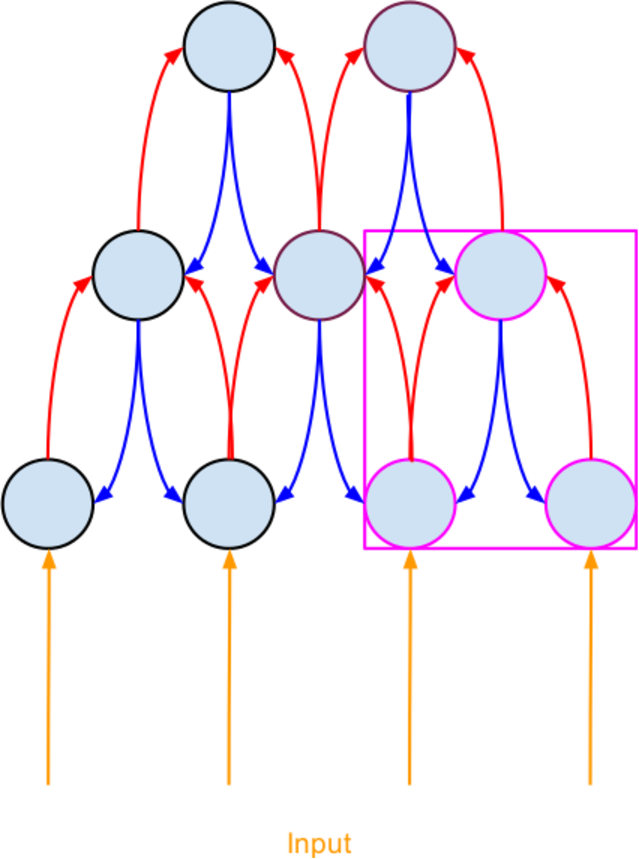
\includegraphics[width=0.5\textwidth]{pictures/perception_predictive_coding}
\end{center}
\end{figure*}

The model that this dissertation adopts is based off of the predictive coding framework \citep{Clark2013}.
In this model, expectations about incoming signal are fed from higher levels of representation to lower ones.
The mismatch between actual perceived signal and the expectations is then propagated back to the higher levels as an error signal.
Future expectations are modified based on the error signal.
This framework captures the basics of perceptual learning, and a similar computational framework has been used to model visually-guided perceptual learning tasks \citep{Kleinschmidt2011}.
However, the attentional mechanism in the predictive coding framework does not work well for some instances of visual attention \citep{Block2013} or for the current results.
I propose a new attentional mechanism for predictive coding, one in which attention inhibits error propagation beyond the level to which attention is directed.
Figures~\ref{fig:predictivecodingperception2} and~\ref{fig:predictivecodingcomprehension2} show schemas reproduced from Chapter~\ref{chap:intro} for perception-oriented and comprehension-oriented attentional sets, respectively.
Such a mechanism explains both the previous findings and the current results.

\begin{figure*}[!ht]
\caption{A schema for predictive coding under a comprehension-oriented attentional set. Attention is represented by the green box, where it is oriented to higher, more abstract levels of sensory representation.  Error signals are able to propagate farther and update more than just the fine grained low level sensory representations. As before, blue errors represent expectations, red arrows represent error signals, and yellow represents the sensory input.}
\label{fig:predictivecodingcomprehension2}
\begin{center}
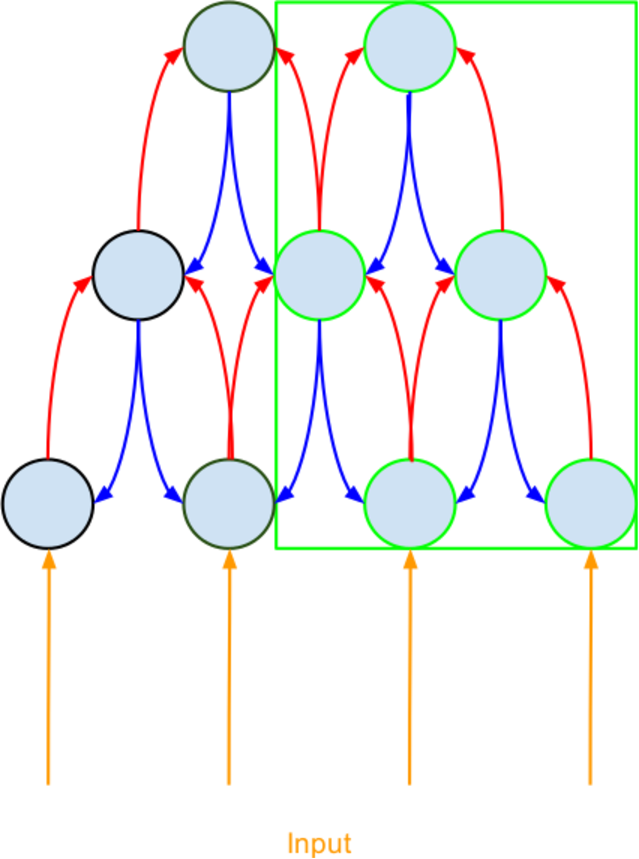
\includegraphics[width=0.5\textwidth]{pictures/comprehension_predictive_coding}
\end{center}
\end{figure*}

The predictive coding framework advanced here has implications for other psycholinguistic research outside of perceptual learning.
Recent innovations in speech perception models have emphasized the role of episodic memory traces \citep{Goldinger1996,Pierrehumbert2001}.
\citet{Theodore2015} argue that attention during encoding can emphasize abstract (i.e. lexical) information at the expense of episodic (i.e., talker) information or vice versa.
Such a proposal is similar to that put forth above, but encoding in a predictive coding framework would be updating of predictions.
The lack of an explicit memory trace mechanism in the predictive coding framework may be a weakness concerning cognition as a whole, but I would argue that it still accounts for the speech perception data.
The primary reason for putting for episodic memory traces originally was to account for behavioral data that showed sensitivity to fine details of previous stimuli \citep{Goldinger1996}.
However, \citet{Sumner2013} highlights recent findings of recognition equivalence but memory inequality between frequent forms and idealized, infrequent forms.
For instance, the word \emph{flute} is generally pronounced with an unreleased /t/ in North American English, but it is also produced less frequently with a fully released /t/ (the idealized form) or with a glottal stop.
All pronunciation variants are recognized equally well in short term processing tasks (accuracy and reaction time).
However, infrequent, idealized pronunciations are remembered better in long term recall tasks.
Sumner and colleagues propose an alternate route to linguistic encoding, what they term socioacoustic encoding.
Hierarchical respresentations with levels along a fine detail to abstract continuum account well for this data without appealing to episodic memory of specific instances.
The socioacoustic encoding would be a speaker-based hierarchical representation, with abstracted gender and accent representations.

While most of the discussion here has concerned representations of speech sounds, predictive coding representations are not solely limited to linguistic objects.
In fact, one of the key findings of perceptual learning is that it is largely dependent on the speaker.
In these cases, perceptual learning is not updating just the distribution for what is expected of a speech sound, but also what is expected for that speaker.
Perceptual learning from a group of speakers that share a trait (i.e., the same non-native accent) facilitates the creation (or perhaps simply the identification) of a more abstract category for that group of speakers, enhancing intelligibility on future novel speakers \citep{Bradlow2008}.

While this dissertation is focused on speech perception, the predictive coding framework can be applied to speech production as well, and in particular sound change.
Individual-level sound change could arise through the generation of an abstract speaker group that conditions a person's perception of speech from that group.
When that person produces speech, they are also perceiving it and compensating for any deviations from their predictions \citep{Hickok2011}.
If the person identifies with the abstract speech group, then the expectations for their own speech will update in accordance to their perception of deviation from that group's speech.

Recent work on a historical vowel change shift in New Zealand English proposed that low frequency words led the shift \citep{Hay2015}.
The mechanism they propose to account for this data is one where tokens that are difficult to comprehend are less likely to be encoded.
Low frequency words are particularly affected because they are likely to be interpreted as higher frequency neighbors and nonwords.
The experiments of this dissertation contained a similar situation at an individual speaker level.
Participants were more likely to not recognize words containing a modified /s/ category as real English words than the filler words.
In Experiment 1, the amount to which a participant's boundary shifted was -- in general -- correlated with the amount of /s/ words recognized as words.
To the extent that difficult to comprehend words are treated as nonwords, these findings reinforce the findings of \citet{Hay2015}.

Outside of psycholinguistcs, this dissertation suggests testable predictions for perceptual learning in the visual domain using visual illusions.
In the Kanizsa illusion, for instance, three Pac-man like objects are arranged to give the illusion of three circles overlaid by a triangle \citep{Kanizsa1976}.
Perception of this illusion requires more abstract representations that are not in the signal, much like the objects of comprehension as defined in this dissertation.
The proposed mechanism for attention would predict that perceptual learning involving visual illusions should be more general and less exposure specific.
In the Kanizsa case, perceivers would perceptually learn characteristics of the abstract triangles and circles instead of the Pac-man shapes.
Visual illusions allow perceivers to better organize complex scenes in short-term and working memory \citep{Vandenbroucke2012}.
Similar to these illusions, words and higher linguistic structures allow better organization of complex auditory signals.
Drawing attention to either the circles and triangles of the illusion or to the Pac-man symbols should induce attentional sets similar to comprehension-oriented and perception-oriented ones proposed in this dissertation, with similar effects on the generalization of perceptual learning.

I have argued that attentional sets, particularly within the predictive coding framework, are crucial to the generalization of perceptual learning to new contexts.
Recent advancements in models of speech perception have been to treat linguistic representations as a balance of both more abstract elements and more fine-detailed elements \citep{Theodore2015} and to incorporate aspects of social representations \citep{Szakay2012, Sumner2013}.
Both of these trends are easy to incorporate into a predictive coding framework.
Such a model accounts for the findings of this thesis and those of the larger psycholinguistic literature.


%\begin{figure*}[!ht]
%\caption{Kanizsa triangle formed by three Pac-man symbols.}
%\label{fig:kanizsa}
%\begin{center}
%
\includegraphics[width=0.3\textwidth]{pictures/Kanizsa}
%\end{center}
%\end{figure*}

%The findings of this thesis relate to theoretical models of speech perception.  
%Predictive coding is a domain-general model of cognition that explicitly incorporates expectation updating \citep{Clark2013}.
%Models of speech perception are more domain-specific and tend to account for phenomena in word recognition.
%Exemplar theoretic frameworks have episodic traces as the primary component, with more abstract representations created through the average of those episodic traces \citep{Pierrehumbert2002}.


\section{Conclusion}

This dissertation investigated the influences of attention and linguistic salience on perceptual learning in speech perception.
Perceptual learning was modulated by the attentional set of the listener.
Perception-oriented attentional sets were induced through increasing the salience of the modified category, either by reducing the lexical bias, increasing the typicality, or giving explicit instructions.
In all these instances, participants showed smaller, but still robust perceptual learning effects.
Exposure to modified categories in predictive sentences resulted in no perceptual learning effects, potentially due to the attribution of the modified sound category to reduced speech clarity.
These results support a greater role of attention than previously assumed in predictive coding frameworks, such as the proposed propagation-blocking mechanism.
Finally, these results suggest that the degree to which listeners perceptually adapt to a new speaker is under their control to the same degree as attentional set adoption.
However, given the robust perceptual learning effects found across experiments, perceptual learning is a largely automatic process when variation cannot be attributed to contextual factors.


